%%%%%%%%%%%%%%%%%%%%%%% file template.tex %%%%%%%%%%%%%%%%%%%%%%%%%
%
% This is a general template file for the LaTeX package SVJour3
% for Springer journals.          Springer Heidelberg 2010/09/16
%
% Copy it to a new file with a new name and use it as the basis
% for your article. Delete % signs as needed.
%
% This template includes a few options for different layouts and
% content for various journals. Please consult a previous issue of
% your journal as needed.
%
%%%%%%%%%%%%%%%%%%%%%%%%%%%%%%%%%%%%%%%%%%%%%%%%%%%%%%%%%%%%%%%%%%%
%
% First comes an example EPS file -- just ignore it and
% proceed on the \documentclass line
% your LaTeX will extract the file if required
\begin{filecontents*}{example.eps}
%!PS-Adobe-3.0 EPSF-3.0
%%BoundingBox: 19 19 221 221
%%CreationDate: Mon Sep 29 1997
%%Creator: programmed by hand (JK)
%%EndComments
gsave
newpath
  20 20 moveto
  20 220 lineto
  220 220 lineto
  220 20 lineto
closepath
2 setlinewidth
gsave
  .4 setgray fill
grestore
stroke
grestore
\end{filecontents*}
%
\RequirePackage{fix-cm}
%
%\documentclass{svjour3}                     % onecolumn (standard format)
%\documentclass[smallcondensed]{svjour3}     % onecolumn (ditto)
%\documentclass[smallextended]{svjour3}       % onecolumn (second format)
\documentclass[twocolumn]{svjour3}          % twocolumn
%
\smartqed  % flush right qed marks, e.g. at end of proof
%
\usepackage{graphicx}
%
\usepackage{mathptmx}      % use Times fonts if available on your TeX system
%
% insert here the call for the packages your document requires
%\usepackage{latexsym}
% etc.
%
\usepackage{natbib} % [numbers]
\usepackage{hyperref}



\usepackage{booktabs}
\usepackage{multirow}
\usepackage{tabularx}
\usepackage{longtable}
\usepackage{lipsum}
\usepackage{lscape}
\usepackage{siunitx}
\usepackage{amsmath}
%\usepackage{cleveref}
% please place your own definitions here and don't use \def but
% \newcommand{}{}
%
% Insert the name of "your journal" with
\journalname{Energy Efficiency}
%
\begin{document}

\title{Air Compressor Mode Identification Using Real-Time Clustering Methods for Efficiency Degradation Detection%\thanks{Grants or other notes
%about the article that should go on the front page should be
%placed here. General acknowledgments should be placed at the end of the article.}
}
%\subtitle{Do you have a subtitle?\\ If so, write it here}

%\titlerunning{Short form of title}        % if too long for running head

\author{Se\'an Martin Hayes         \and
        D.T.J. O'Sullivan %etc.
}

%\authorrunning{Short form of author list} % if too long for running head

\institute{Se\'an Martin Hayes \and D.T.J. O'Sullivan \at
              School of Engineering \\
              University College Cork \\
              Ireland \\
              Tel.: +353-21-4902913\\
              Fax: +353-21-4276648\\
              \email{sean.m.hayes@umail.ucc.ie}           %  \\
%             \emph{Present address:} of F. Author  %  if needed
           \and
 %          S. Author \at
  %            second address
}

\date{Received: date / Accepted: date}
% The correct dates will be entered by the editor


\maketitle

\begin{abstract}
Insert your abstract here. Include keywords, PACS and mathematical
subject classification numbers as needed.
\keywords{First keyword \and Second keyword \and More}
% \PACS{PACS code1 \and PACS code2 \and more}
% \subclass{MSC code1 \and MSC code2 \and more}
\end{abstract}

\section{Introduction}
\label{intro}

In 2012 industry consumed 2,542 Mtoe of energy globally, which represented  over 28\% of the 8,980 Mtoe of global final energy consumption \cite{IEA2012}. In an Irish context, industry consumed 2.26 Mtoe of energy in 2012, representing almost 22\% of Ireland’s 10.3 Mtoe of final energy consumption. Within the category of industrial energy, compressed air is recognised as an energy intensive utility, accounting for 10\% of industrial electricity in the European Union \cite{Saidur2010}. Energy costs typically account for 78\% of the total life cycle cost of a compressed air system \cite{radgen2006efficiency}. Compressed air is known colloquially in industry as the “fourth fuel”, due to the high electrical cost associated with generation. Compressed air systems are typically running at 19\% overall system efficiency \cite{Saidur2010}, due to energy losses largely due to lost heat of generation and leakages.

Compressed air has been recognised as having significant energy saving potential in the food industry \cite{Wang2014}, not least through measures such as retrofitting of variable speed drives, inlet air temperature reduction, waste heat recovery, and pressure and leakage reduction (cite Wang 2008 from Wang 2014 paper).

\section{Thermodynamics of Air Compression}
The thermodynamics of air compression are outlined in \autoref{fig:thermocomp}.

\begin{figure}
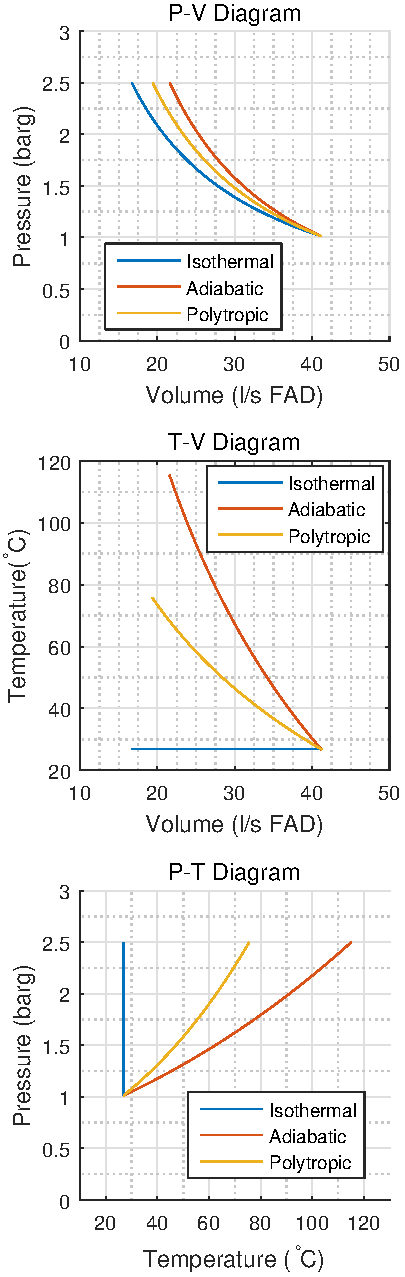
\includegraphics[height = \textheight]{./Images/Compression_ThermoDiagrams.pdf}
\caption{Thermodynamics of Air Compression}
\label{fig:thermocomp}
\end{figure}



\section{Determining the operational performance of an air compressor}
\label{sec:probstatement}
A wide range of configurations and types of compressed air systems are installed in industry. In many cases there exist systems which are running sub-optimally, either due to unsuitability for the task at hand or running in a faulty condition. Given that compressed air represents such a dense form of energy transport, it is beneficial in terms of long and short term overall energy efficiency goals to manage the performance of air compressors. Performance management is typically achieved through means such as those in  \autoref{tab:perfmgmt}. The key disadvantages of existing methods are either that they are manual and periodic in nature, or that they require the intervention of a human expert in compressed air systems to be effective. In the case of maintenance contracts and periodic audits, there is also the potential for unnecessary work to be carried out, as both these measures are typically carried out on a timescale basis. The intervention of a human expert also lends itself to an inefficient method of performance measurement. An expert may be particularly well versed with one type of system, but not another. The disparate range of compressed air systems can lead to an expert restricting themselves to one type of system, preventing possible lessons learned to be applied in other suitable cases.

% Table generated by Excel2LaTeX from sheet 'Sheet1'
\begin{table}
  \centering
  \caption{Existing Compressed Air System Performance Management Methods}
    \begin{tabular}{p{.3\linewidth}p{.3\linewidth}p{.3\linewidth}}
    \toprule
    Performance Management Method & Advantages & Disadvantages \\
    \midrule
    Maintenance Contracts & Security of asset reliability & Potential for unnecessary work \\
    Periodic Audits & Likely to pick up on common opportunities for improvement & Dependent on skill level of auditor \\
    Sequence Controllers & Can draw on manufacturer knowledge of system operation & Initial configuration may not be maintained due to system changes \\
    BMS Monitoring & Desk-based site wide monitoring capability & Dependent on skill level of BMS reviewer. Unable to pick up on sensor errors \\
    \bottomrule
    \end{tabular}%
  \label{tab:perfmgmt}%
\end{table}%


%	Bumph about current methods to detect performance degradation

In order to analyse a particular compressed air system it is useful to understand how it might relate to other installations. The system analysed in this paper consists of two rotary tooth air compressors with a heated desiccant dryer, with the layout given in \autoref{fig:compairlayout}. These machines are rotary tooth type machines, which are widely deployed across industry for applications with medium pressure and capacity requirements, as shown in \autoref{fig:CompApps}\cite{SEAI2007} The various types of compressors typically used in industry are shown in \autoref{fig:comptypes}. Reciprocating and rotary machines are both positive displacement type machines. They work through isolation of a quantity of air in a space which is then reduced in volume. Centrifugal machines are aerodynamic machines, which operate by imparting kinetic energy to air, which is then converted to pressure energy by stopping the moving air. The three most common types of compressor in industry are rotary, reciprocating and centrifugal machines. The application ranges of these types are shown in \autoref{fig:CompApps} \cite{SEAI2007}.

\begin{figure*}
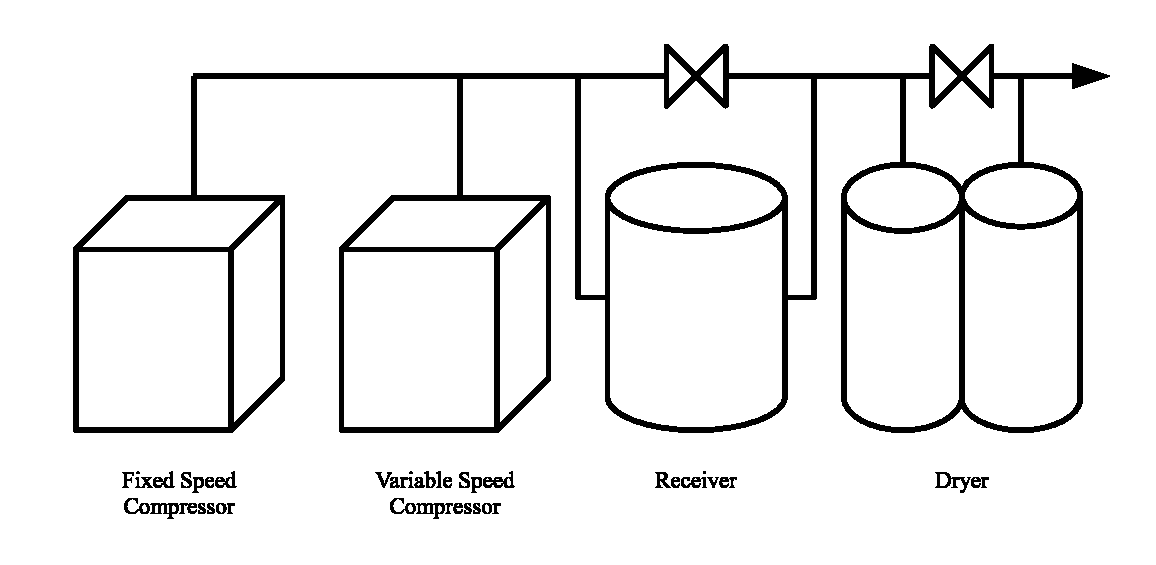
\includegraphics[width = \textwidth]{./Images/PharmacyCompAir.eps}
\caption{Test Site Compressed Air System Layout}
\label{fig:compairlayout}
\end{figure*}

\begin{figure}
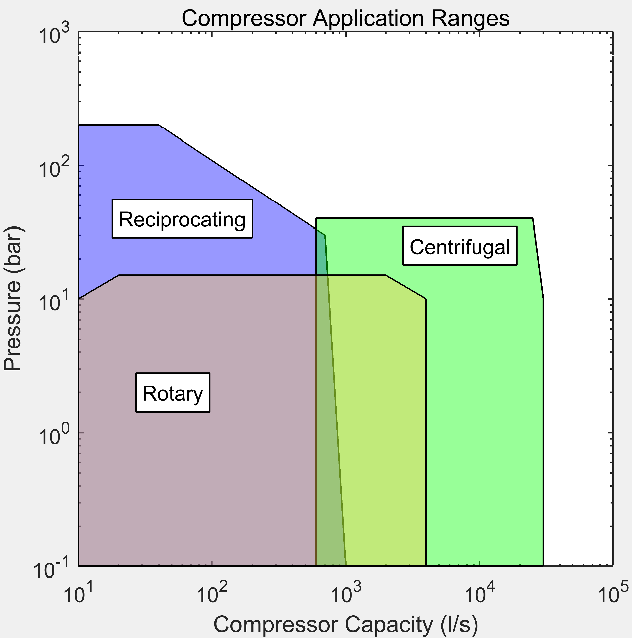
\includegraphics[width = \columnwidth]{./Images/CompApps.pdf}
\caption{Compressor Application Suitability}
\label{fig:CompApps}
\end{figure}
\begin{figure*}

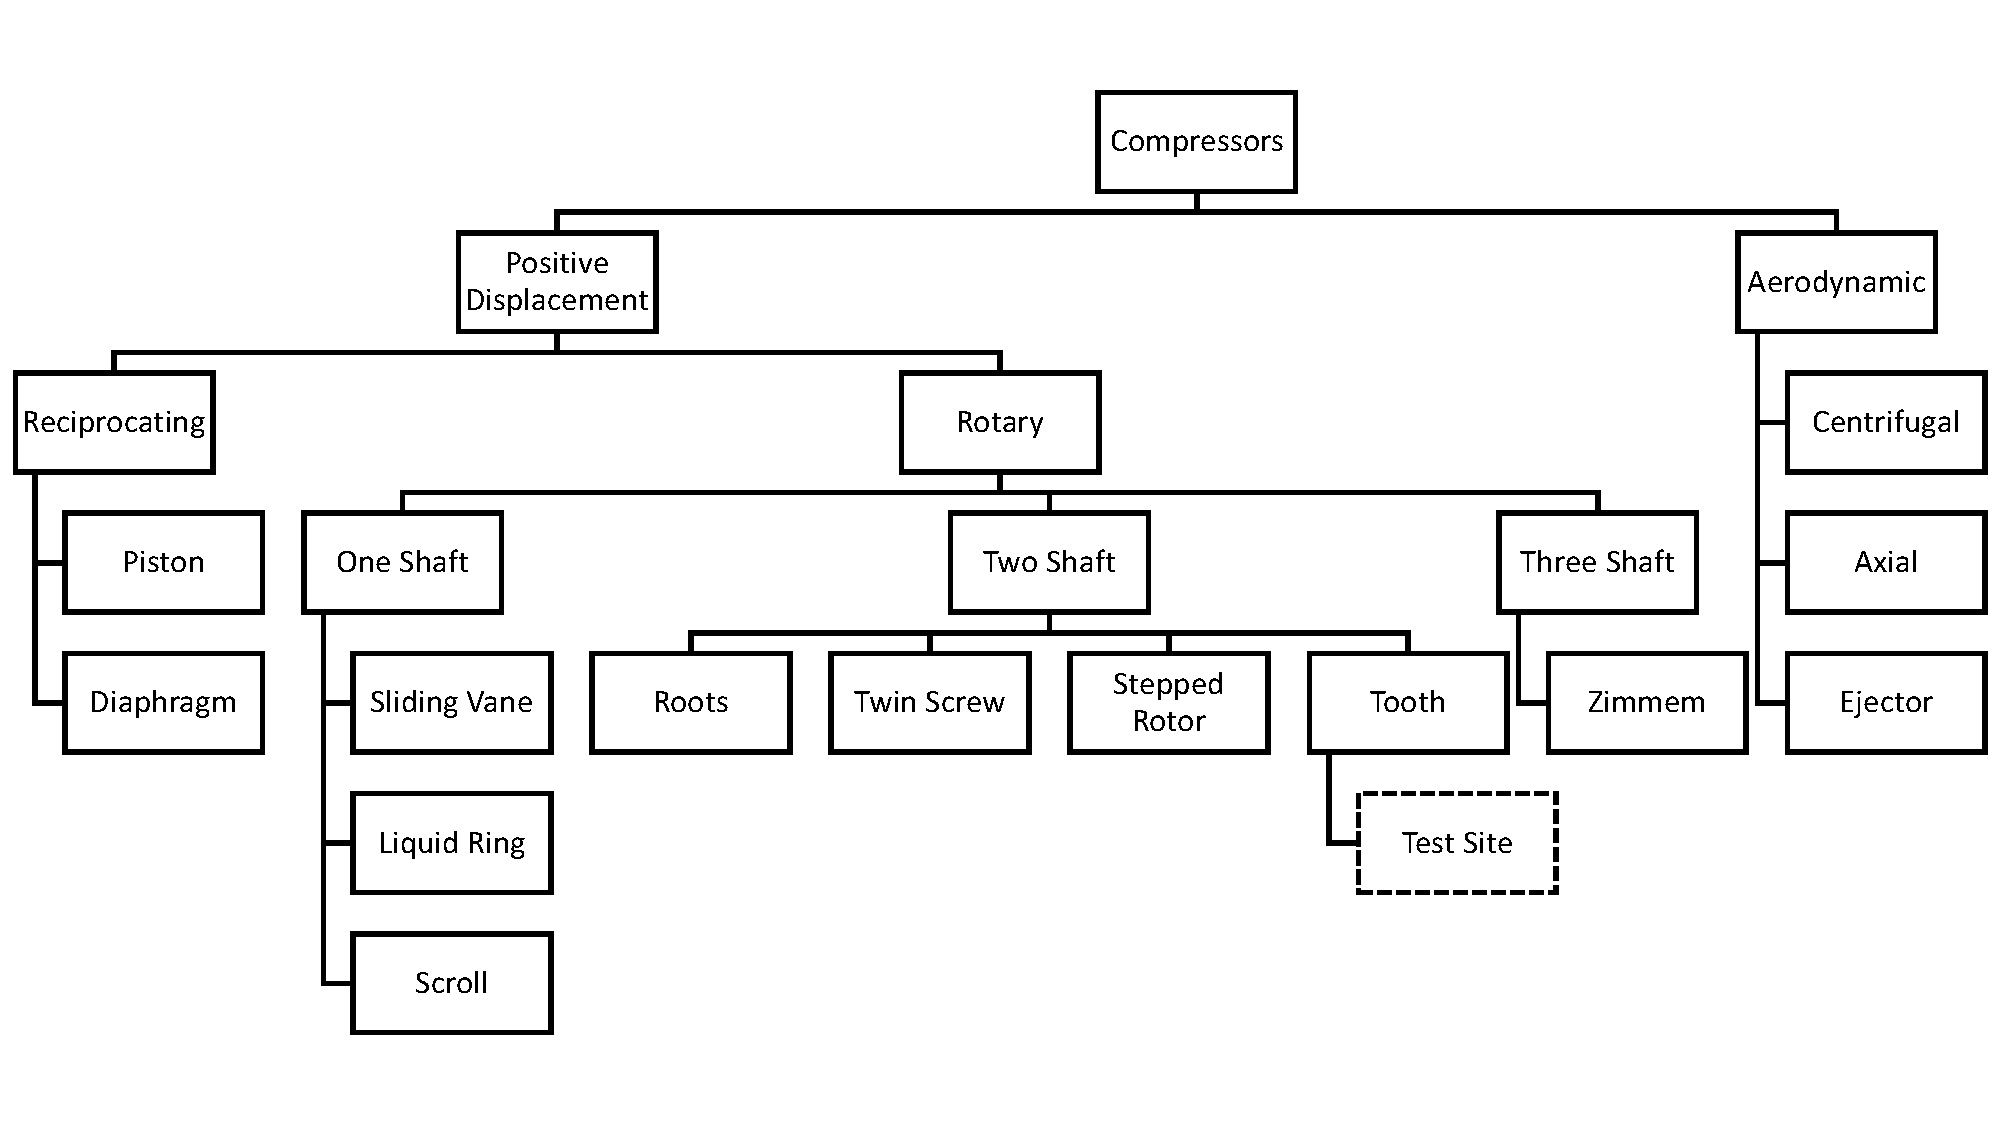
\includegraphics[width = \textwidth]{./Images/CompressorClassification.pdf}
\caption{Compressor Types}
\label{fig:comptypes}
\end{figure*}

Research is being carried out to define the future of compressed air system performance management. In this review the research considered is that of ongoing analysis of compressed air system data. This ongoing analysis could be designated as having any of the goals outlined in \autoref{tab:goalsmgmt}.

% Table generated by Excel2LaTeX from sheet 'Sheet2'
\begin{table}
  \centering
  \caption{Goals of Performance Management}
    \begin{tabular}{p{.3\linewidth}p{.3\linewidth}p{.3\linewidth}}
    \toprule
    Goal  & Description & Example Work \\
    \midrule
    Fault Detection and Diagnosis & Monitor system parameters to determine when system is in fault condition and the potential reasons for the identified fault & Using vibration, pressure and current signals to diagnose valve faults for a reciprocating compressor \cite{Tran2014} \\
    Prognostics & Monitoring system parameters to determine when a component of a system will no longer perform its intended function \cite{Vachtsevanos2006} & Determining the remaining useful life of a gaseous circuit breaker  based on gas pressure and ambient temperature \cite{Catterson2013} \\
    Analytics & Monitoring system parameters to discover meaningful patterns which may advise on potential improvements to system operation & Determining abnormal appliance power consumption based on analysis of individual appliance’s acoustic noise \cite{Pathak2015} \\
    Automated Commissioning & Achieving, verifying and documenting that the performance of a system satisfies the current user requirement & Automatically carrying out the normal testing procedure for an air compressor by replicating the tasks normally carried out during commissioning \cite{Mazid2008} \\
    Optimisation & Improving system operation or design as measured against some defined criteria & Development of a tool which delivers an optimal design for a compressed air system based on energy and life cycle costing \cite{Friden2012} \\
    Control & Managing the operation of a system in order that operating conditions remain in line with design states and undesirable states are avoided & Development of a control algorithm for fixed speed compressors that provides the pressure control capabilities of a variable speed system while limiting energy consumption \cite{Facchinetti} \\
    \bottomrule
    \end{tabular}%
  \label{tab:goalsmgmt}%
\end{table}%

\subsection{Current research into performance management}
\label{subsec:perfmgmtmethods}
\autoref{fig:perfmgmtmethods}.

\begin{figure*}
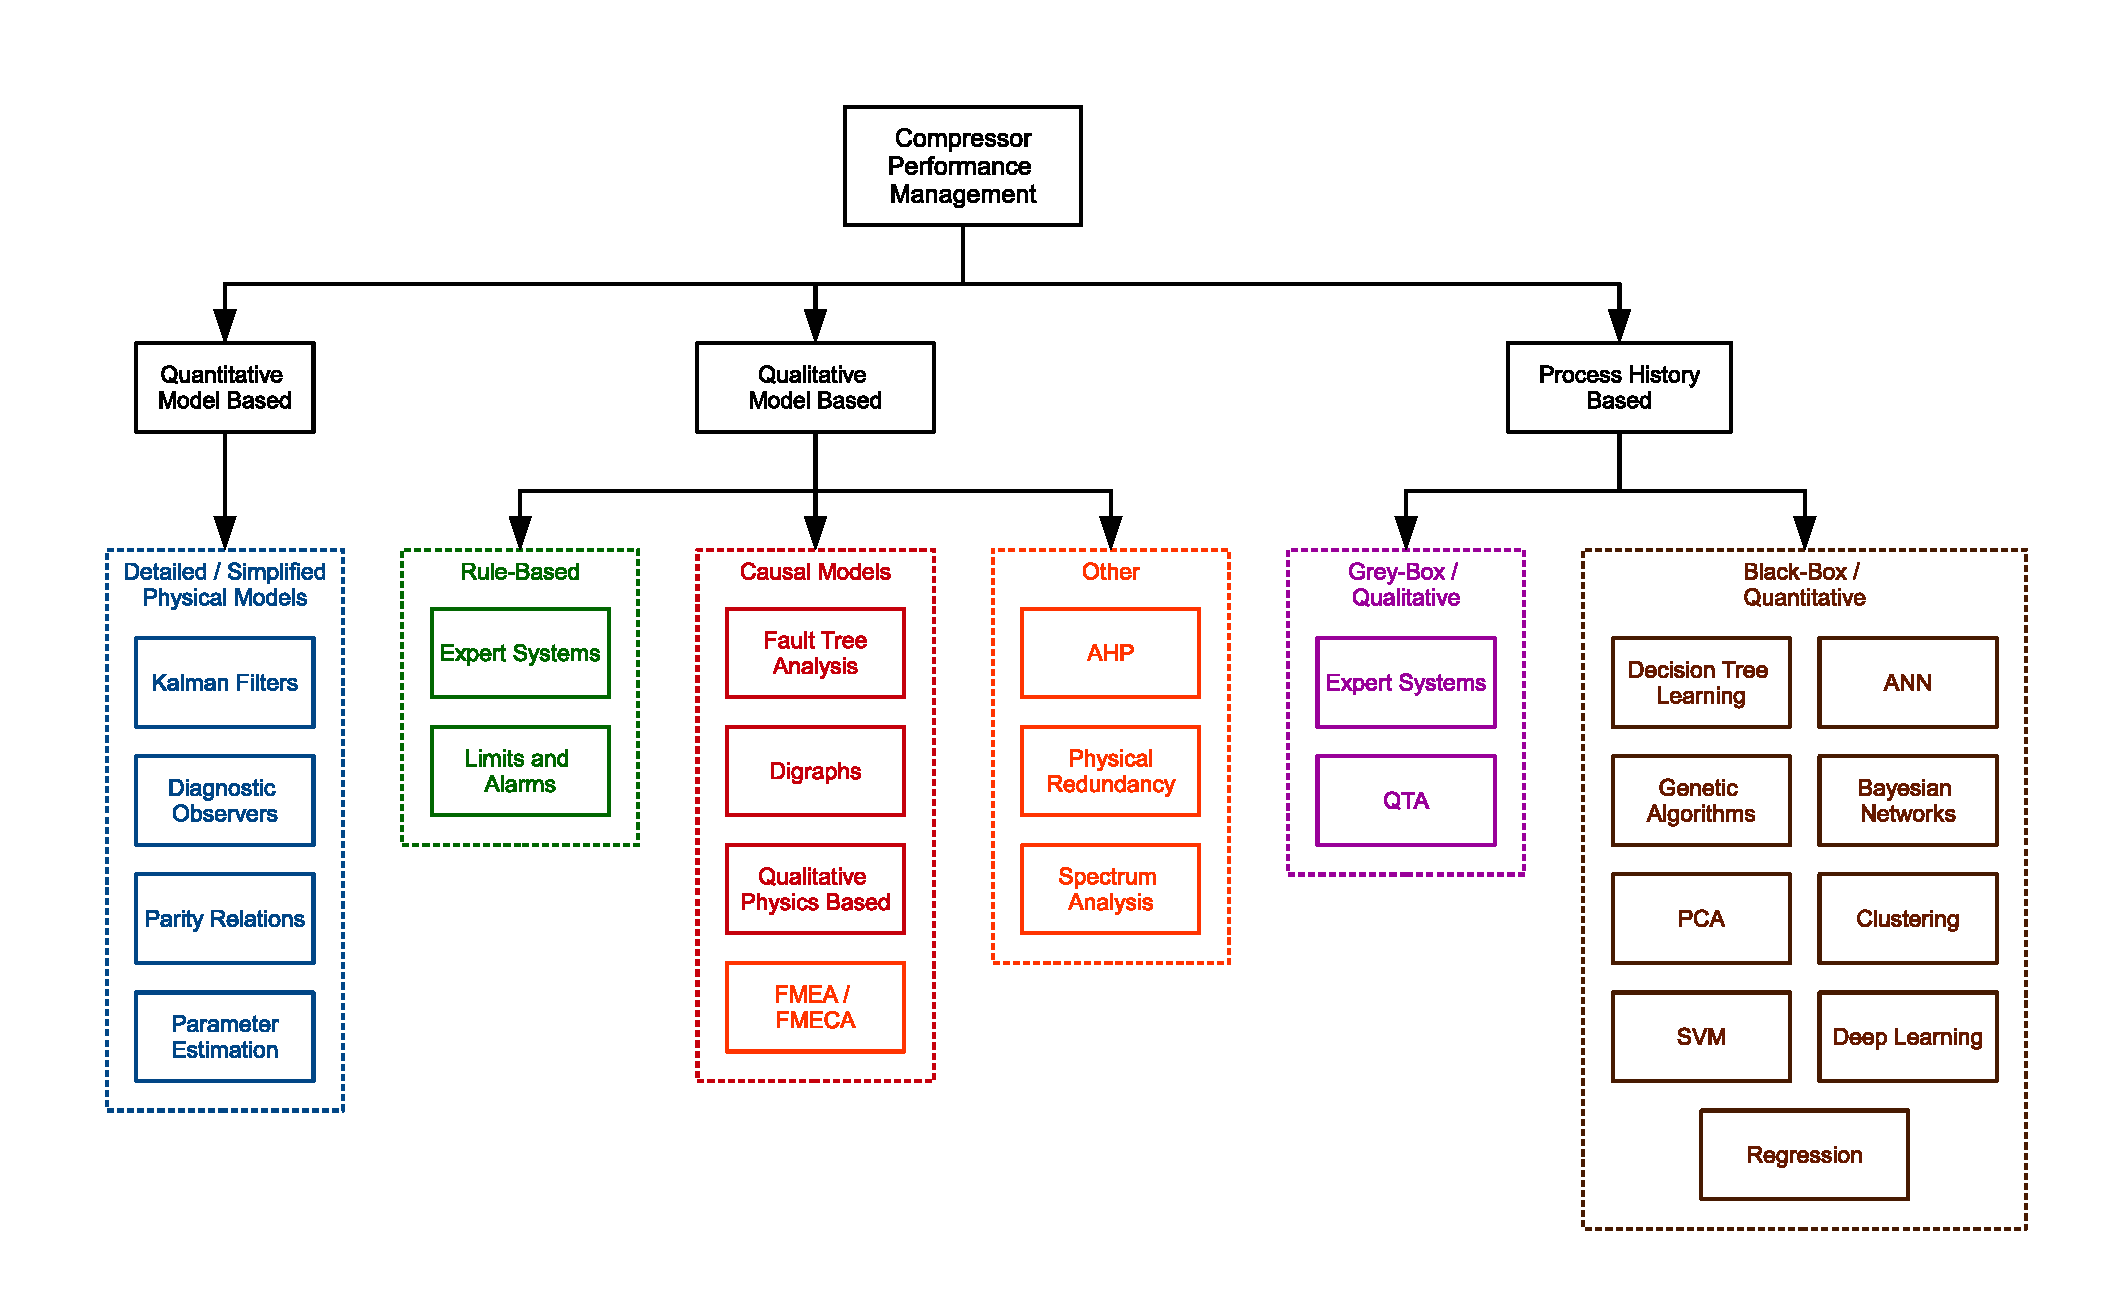
\includegraphics[width=\textwidth]{./Images/perfmgmt.eps}
\caption{Current research into performance management methods}
\label{fig:perfmgmtmethods}
\end{figure*}

Quantitative model based methods are summarised in ...

\begin{table*}
\caption{Quantitative model based methods}
\begin{tabular}{p{.18\textwidth}p{.18\textwidth}p{.18\textwidth}p{.18\textwidth}p{.18\textwidth}}
\toprule
Method &	Description&	Benefits&	Disadvantages&	Examples \\
\toprule
\multirow{4}{.18\textwidth}{Kalman Filters} &\multirow{4}{.18\textwidth}{A Kalman filter allows the combination of observed and predicted parameters to more accurately predict future parameters than with a physical model alone. It also allows for the reduction of the effects of noisy data on models.} & Very accurate&	Computationally expensive&	Surge control for axial compressors \cite{Backi2013}\\
&  &  Transients may be modelled&	Complex to create&	Fault detection for gas turbine compressors \cite{Salar2010} \\
& & & Typically require many inputs from system	&State estimation of a thermal power plant \cite{Nair2011})\\
& & & & Leakage detection of a pneumatic network \cite{Krichel2011}\\
\midrule
\multirow{3}{.18\textwidth}{Diagnostic Observers} & \multirow{3}{.18\textwidth}{Employing state observers, typically one for each fault, which represent a different output from a model, in order that observed differences in outputs may be attributed to faults to how to change a model to remove deviations from expected behaviour} & Accurate isolation of individual faults possible &	Observers required for each individual potential fault state &	Fault detection of a steam boiler feed water preheater \cite{Tarantino2000}\\
 & & & & Estimation of a steam boiler’s pressure given fuel and feed water conditions \cite{Ramezanifar2006}\\
 & & & & Surge control for axial compressors \cite{Backi2013}\\
 \midrule
Parity Relations &	Rearranging and transforming input-output models of a system in order to highlight individual fault conditions &	Accurate isolation of individual faults possible &	Less effective at identifying multiplicative faults &	Fault diagnosis of a wind farm using interval nonlinear parameter-varying parity equations \cite{Blesa2014}\\
\midrule
Parameter Estimation & Comparison of modelled data, normally using ordinary and partial differential equations, with measured data, with analysis of any residuals to diagnose faults
 & High level of confidence in modelled data & Detailed physical model required for accuracy & Optimisation of the modelling of a multistage compressor using parameter estimation to determine the surge line \cite{DapengNiu2011} \\
\bottomrule
\end{tabular}
\label{tab:quantimodel}
\end{table*}

% Table generated by Excel2LaTeX from sheet 'Sheet2'
\begin{table*}[htbp]
  \centering
  \caption{Qualitative model based methods}
    \begin{tabular}{p{.18\textwidth}p{.18\textwidth}p{.18\textwidth}p{.18\textwidth}p{.18\textwidth}}
    \toprule
    Method & Description & Benefits & Disadvantages & Examples \\
    \midrule
    Expert Systems & Using if-then-else rules derived from engineering knowledge of a system’s operation to flag when and why a fault is present in operation & Quick deployment potential & Potential that knowledge remains undiscovered/undocumented & Fault diagnosis assistance using IF-THEN rules for an air compressor \cite{Liu2001}\\
    \midrule
    Physical Redundancy & Installing parallel sensors in order that site personnel be notified of an error if sensor values do not match & Simple in concept & Cost and space constraints may limit additional sensor placement & Analysis framework of fault detection schemes based on redundant sensors for aircraft \cite{Wheeler2011}\\
    \midrule
    Analytical Hierarchy Process & Decision support for selection of a particular approach, e.g. for maintenance strategy, over another based on pairwise comparisons of suitability toward various goals & Allows documentation of expert decision making in formal manner & Limited real-time performance analysis potential & Maintenance strategy selection for equipment at an oil refinery \cite{Bevilacqua2000}\\
    \midrule
    Spectrum Analysis & Analysis of compressor drive and vibrational frequency response to alert when response drifts from normal & Allows for discovery of faults which may be difficult to postulate from first principles & Detailed analysis required for each potential spectrum case & Vibration analysis of reciprocating compressors for valve failure diagnosis \cite{RuilinLin2010}\\
    \midrule
    Fault Tree Analysis & Postulation of potential areas of failure in equipment & Allows formal documentation of human expert knowledge & Scope of fault detection is as limited as human expert’s knowledge and expertise & Reliability assessment of an anti-surge control system for a centrifugal compressor \cite{Ren2012}\\
    \midrule
    FMEA / FMECA & Analysis of site equipment potential areas of failure and potential effect on other equipment & Critical analysis of most risk-prone areas of a system & Time consuming for development & Compressor safety evaluation model \cite{Zhu2013}\\
    \midrule
    Qualitative Physics Based & Derivation of qualitative equations from fundamental physical equations governing system operation to allow for analysis without explicit requirement for numerical values & No requirement for numerically accurate measurement of system variables & Requires initial understanding of physical processes governing system operation & Fault Detection for an AHU \cite{Glass1995}\\
    \midrule
    Digraphs & Representation of qualitative models using directed graphs to efficiently incorporate system behaviour for effective analysis & Allows visual representation of qualitative physical equations & Requires considerable domain expertise for creation & FDD for a typical industrial process using SDG for model decomposition \cite{Shin2007}\\
    \midrule
    \multicolumn{1}{c}{\multirow{2}[0]{.18\textwidth}{Limits and Alarms}} & \multicolumn{1}{c}{\multirow{2}[0]{.18\textwidth}{Implementation of user defined limits on key parameters which flag when exceeded or are not met}} & \multicolumn{1}{c}{\multirow{2}[0]{.18\textwidth}{With correct identification of thresholds can quickly highlight issues with systems}} & Little diagnosis and isolation potential & \multicolumn{1}{c}{\multirow{2}[0]{.18\textwidth}{Incorporated into modern compressor PLCs}} \\
    \multicolumn{1}{c}{} & \multicolumn{1}{c}{} & \multicolumn{1}{c}{} & Correct selection of thresholds dependent on user expertise & \multicolumn{1}{c}{} \\
    \bottomrule
    \end{tabular}%
  \label{tab:qualimodel}%
\end{table*}%




\onecolumn
% Table generated by Excel2LaTeX from sheet 'Sheet3'
  \begin{center}
    \begin{longtable}{p{.18\textwidth}p{.18\textwidth}p{.18\textwidth}p{.18\textwidth}p{.18\textwidth}}
    \caption[Process history based methods]{Process history based methods} \label{tab:prochist} \\
    \toprule
    Method & Description & Benefits & Disadvantages & Examples \\
    \toprule 
    \endfirsthead
    
    \multicolumn{5}{c}%
    {{ \tablename\ \thetable{} -- continued from previous page}} \\
    \toprule
    Method & Description & Benefits & Disadvantages & Examples \\
    \toprule 
    \endhead
    
    Support Vector Machine / Relevance Vector Machine & A supervised learning technique which when given a sample data set which is labelled according to which class each point belongs in, can determine the optimal plane which splits classes allowing accurate future classification of variables & Can accurately classify non-linear data & Can be computationally expensive in implementation & Compressed air load forecasting for large flows \cite{Liu2013};  Fault diagnosis for reciprocating air compressor valves \cite{Wang2010}, \cite{Cui2009}, \cite{Qin2012}, \cite{JamesLi1995}; Fault diagnosis for reciprocating air compressors \cite{Verma2011} \\

    \midrule
    
    \multirow{3}[0]{.18\textwidth}{PCA} & \multirow{3}[0]{.18\textwidth}{Analysis of a population of variables to determine the population extremes in a given number of directions or components, allowing categorisation of each data point in terms of its position in each direction} & Decreased sensitivity of data analysis to noise & \multirow{3}[0]{.18\textwidth}{Training data must explicitly demonstrate variance in data} & Sensor fault detection, diagnosis and estimation for centrifugal chillers \cite{Wang2005}\\
    \multicolumn{1}{c}{} & \multicolumn{1}{c}{} & Reduced dimensionality increases data understanding & \multicolumn{1}{c}{} & Fault detection and isolation for a centrifugal compressor \cite{Zanoli2013}\\
    \multicolumn{1}{c}{} & \multicolumn{1}{c}{} &       & \multicolumn{1}{c}{} & Sensor and actuator fault diagnosis for a centrifugal compressor \cite{Zanoli2010a}\\
    \midrule
    
        
    \multicolumn{1}{c}{\multirow{4}[0]{.18\textwidth}{Artificial Neural Networks}} & \multicolumn{1}{c}{\multirow{4}[0]{.18\textwidth}{Creation of a network of elements or neurons which may determine output values based on interconnected element's response to external inputs. Networks may be supervised where instances of faulty operation are labelled, allowing the network to generate expected outputs for arbitrary unknown inputs. Networks may also be unsupervised, in which case the topology is adaptively determined based on the inputs.}} & \multicolumn{1}{c}{\multirow{4}[0]{.18\textwidth}{Can effectively predict non-linear relationships in data}} & \multicolumn{1}{c}{\multirow{4}[0]{.18\textwidth}{Structure of neural network requires intuitive development}} & Valve failure detection for reciprocating compressors (Namdeo et al. 2008) \\
    \multicolumn{1}{c}{} & \multicolumn{1}{c}{} & \multicolumn{1}{c}{} & \multicolumn{1}{c}{} & Neural network based fault diagnosis of a reciprocating compressor employing genetic algorithms for initial parameter identification \cite{Jinru2008}\\
    \multicolumn{1}{c}{} & \multicolumn{1}{c}{} & \multicolumn{1}{c}{} & \multicolumn{1}{c}{} & Performance prediction of a centrifugal air compressor employing artificial neural networks and genetic algorithms \cite{LuoFangqiong2011}\\
    \multicolumn{1}{c}{} & \multicolumn{1}{c}{} & \multicolumn{1}{c}{} & \multicolumn{1}{c}{} & Generation of a gas generator’s compressor performance characteristic map \cite{Ghorbanian2009} \cite{Yu2007}\\
    \midrule
    \multicolumn{1}{c}{\multirow{4}[0]{.18\textwidth}{Genetic Algorithms}} & \multicolumn{1}{c}{\multirow{4}[0]{.18\textwidth}{Determining the optimum point a system can operate at, by selecting random members of a population of samples and using them as parents of successive samples, which tend toward the optimal sample}} & \multicolumn{1}{c}{\multirow{4}[0]{.18\textwidth}{Easily transferred to existing simulations and  models}} & \multicolumn{1}{c}{\multirow{4}[0]{.18\textwidth}{No assurance that optimal application will indeed be the global optimum}} & Noise minimisation of a hermetic compressor \cite{Dasilva2004}\\
    \multicolumn{1}{c}{} & \multicolumn{1}{c}{} & \multicolumn{1}{c}{} & \multicolumn{1}{c}{} & Neural network based fault diagnosis of a reciprocating compressor employing genetic algorithms for initial parameter identification \cite{Jinru2008} \\ %
    \multicolumn{1}{c}{} & \multicolumn{1}{c}{} & \multicolumn{1}{c}{} & \multicolumn{1}{c}{} & Performance prediction of a centrifugal air compressor employing artificial neural networks and genetic algorithms \cite{LuoFangqiong2011}\\
    \multicolumn{1}{c}{} & \multicolumn{1}{c}{} & \multicolumn{1}{c}{} & \multicolumn{1}{c}{} & Parameter identification for a centrifugal compressor model \cite{Xiaogang2013}\\
    \midrule
    Decision Tree Learning & Automatic classification of output variables by organising data into subsets, generating rules in a tree like structure & Require reasonably low data preparation effort & Highly unstable when perturbations in training data are present & Fault diagnosis for a modular production system \cite{Demetgul2013}\\
    \midrule
    Deep Belief Networks & Stacked Restricted Boltzmann Machines (RBMs), which are themselves simple unsupervised neural networks & Allow more complex understanding of data relationships than with lower level machine learning techniques & Complex to initially understand structure & Reciprocating compressor valve fault diagnosis \cite{Tran2014}\\
    \midrule
    \multicolumn{1}{c}{\multirow{2}[0]{.18\textwidth}{Clustering}} & \multicolumn{1}{c}{\multirow{2}[0]{.18\textwidth}{Grouping data readings into different groups where intragroup similarity is greater than intergroup similarity}} & \multicolumn{1}{c}{\multirow{2}[0]{.18\textwidth}{Relatively simple to deploy}} & \multicolumn{1}{c}{\multirow{2}[0]{.18\textwidth}{Some qualitative assessment for optimal number of clusters may be required}} & Fault detection and isolation for a centrifugal compressor based on PCA and Clustering \cite{Zanoli2010}\\
    \multicolumn{1}{c}{} & \multicolumn{1}{c}{} & \multicolumn{1}{c}{} & \multicolumn{1}{c}{} & Adaptive clustering for pneumatic system fault detection \cite{Petkovic2012}\\
    \midrule
    \multirow{2}{.18\textwidth}{Bayesian Networks} & \multirow{2}{.18\textwidth}{Creation by learning or using prior knowledge of graphical probabilistic models which give relationships between variables} & \multirow{2}{.18\textwidth}{Can provide an excellent interpolation to real world simulations} & \multirow{2}{.18\textwidth}{Calculation of parameters for Bayesian models can be initially difficult} & Fault diagnosis of a pneumatic air braking system \cite{Lingling2010}\\
          &       &       &       & Fault detection via classification of compressor variables compressed dimensionally via PCA \cite{Liu2009}\\
    \midrule
    Regression Modelling & Statistical estimation of the relationship between two or more variables & Reasonably low effort required for deployment with concept simple to understand & Requires strongly defined relationships between variables to be of any use & Optimisation of a network of compressors in parallel \cite{Kopanos2015} \\ %
    \bottomrule
    \end{longtable}%
\end{center}
% %\end{longtable}%
\twocolumn

\lipsum[1-10]

\section{Rule base development and testing}
\label{sec:rules}
One of the approaches for performance management of air compressors outlined in \autoref{subsec:perfmgmtmethods} is that of Expert Systems. This is a qualitative method which can use rule sets to encode expert knowledge about a system for flagging when a fault in operation is present. This method has been used with success in the case of HVAC (\cite{Bruton2014}, \cite{House2001}) and the area of air compressors (\cite{Liu2001}). Rules for system analysis are typically derived by taking a fundamental engineering overview of the system, and hypothesising potential rules to determine particular faults.

\autoref{fig:compairflow} shows a high level overview of the test site air compressor, which is a two-stage rotary tooth machine. The figure highlights the expected temperature changes as the compressed air is operated on y each fundamental component. These expected operations form the basis for an initial set of rules to flag when the machine is not operating as expected. To illustrate this point the first element of compression is analysed in detail.

Element 1 of the air compressor compresses air from atmospheric pressure (\SI{101325}{\pascal}) to \SI{250000}{\pascal}. When the compressor is at minimum loading, it is designed to produce \SI{41}{\liter \per \second} of free air. It is useful to analyse the thermodynamics of compressing air at this point. \autoref{fig:thermocomp} shows the relevant thermodynamic diagrams for the compression of this volume of air isothermally, adiabatically and polytropically. The air is compressed in a space which is surrounded by ambient air, which is not an ideal heat reservoir. Therefore the isothermal compression case is not valid. The air is not however thermally isolated from its surroundings, therefore the adiabatic case is also not valid. Actual air compression typically follows the polytropic process model, with the polytropic exponent of \autoref{eq:polytropcompression} ranging between 1 and 1.4.

\begin{eqnarray}
\label{eq:polytropcompression}
P_1 V_1^n = P_2 V_2^n \\
\text{where}~P = \text{Absolute pressure (Pa)} \nonumber \\
\text{V} = \text{Absolute volume (m\textsuperscript{3})} \nonumber \\ 
n = \text{Polytropic exponent} \nonumber
\end{eqnarray} 

Given that the compression process taking place is not isothermal, it is logical to expect that the temperature of the compressed air will increase through the first element of compression, in accordance with \autoref{fig:thermocomp}. If a decrease in temperature is observed, then either a failure in the first stage of compression or in a temperature sensor can be determined. This forms the basis for the first rule of the rule set created for compressor performance analysis, which is summarised in INSERT TABLE REF.

Equation for rule 1

\lipsum[1-10]

\autoref{fig:mechcompressor} shows the mechanical layout of a two stage air compressor.

\begin{figure*}
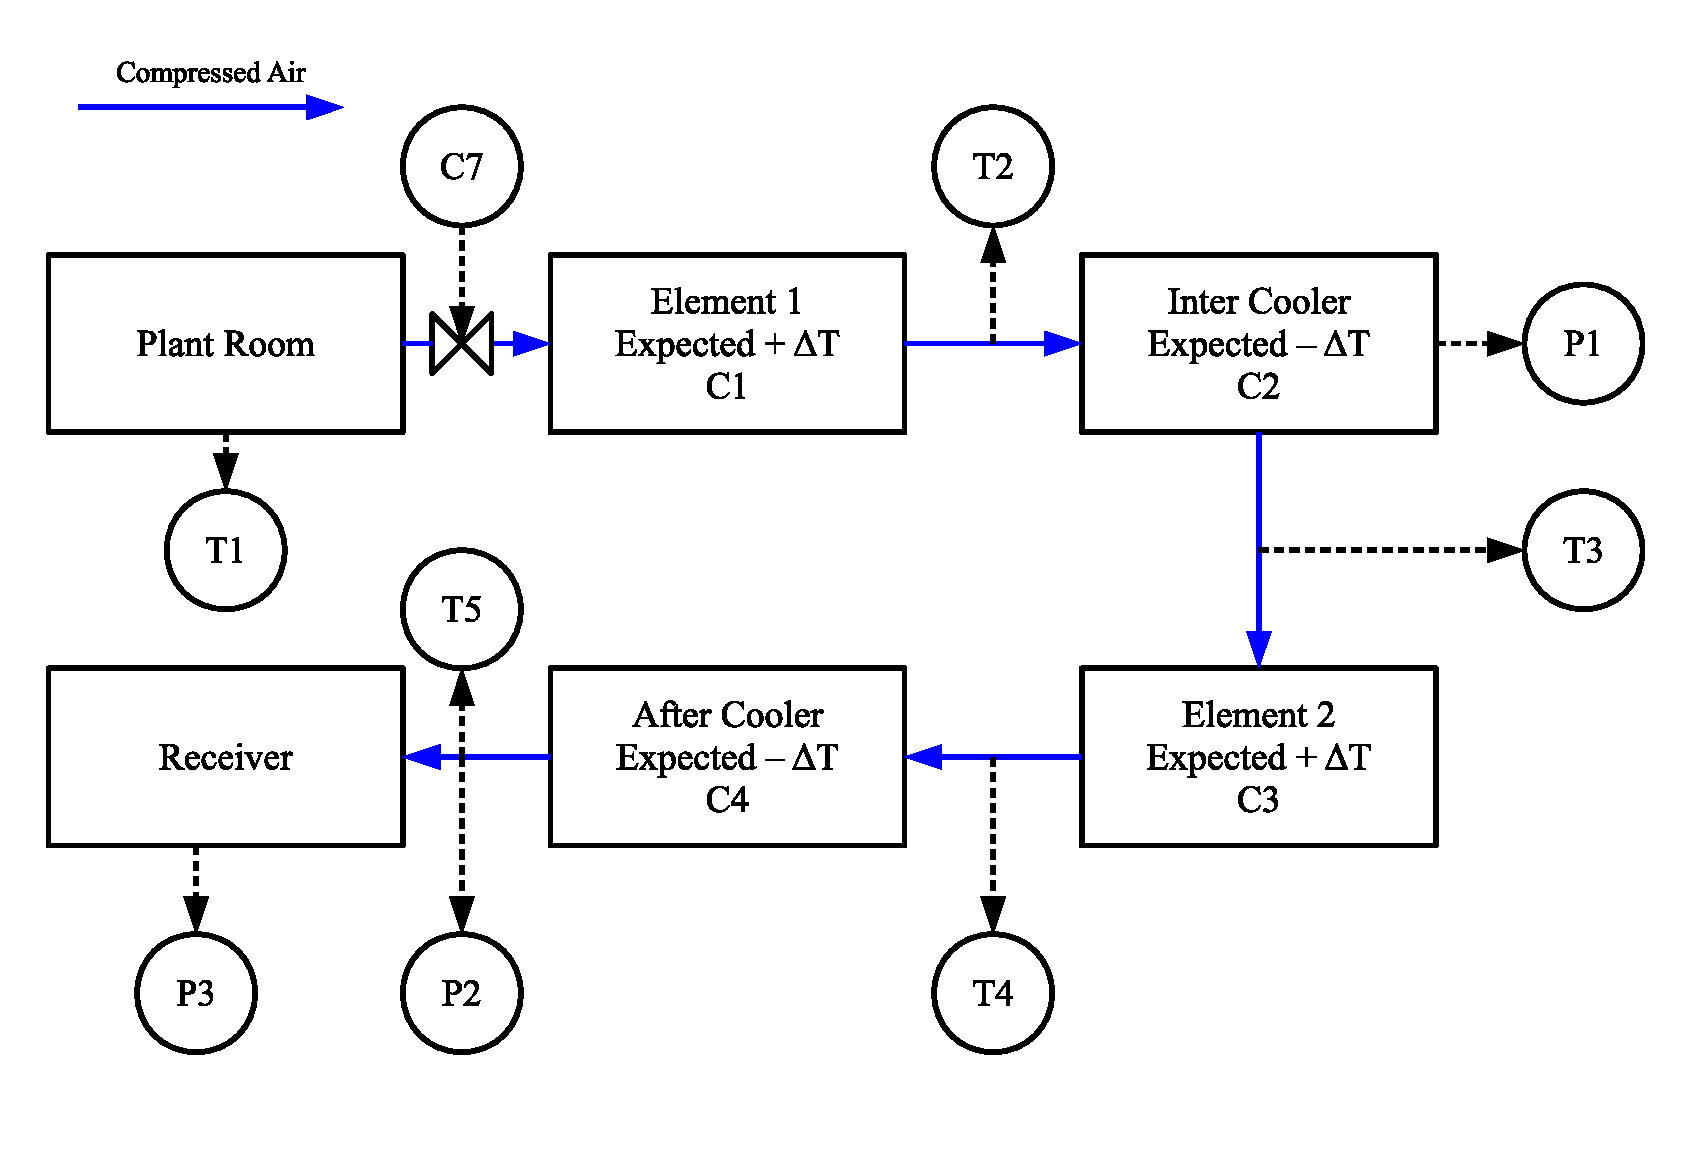
\includegraphics[width = \textwidth]{./Images/2StageRotaryCompressorIdeal.eps}
\caption{Two stage compressor air flow}
\label{fig:compairflow}
\end{figure*}


\begin{figure*}
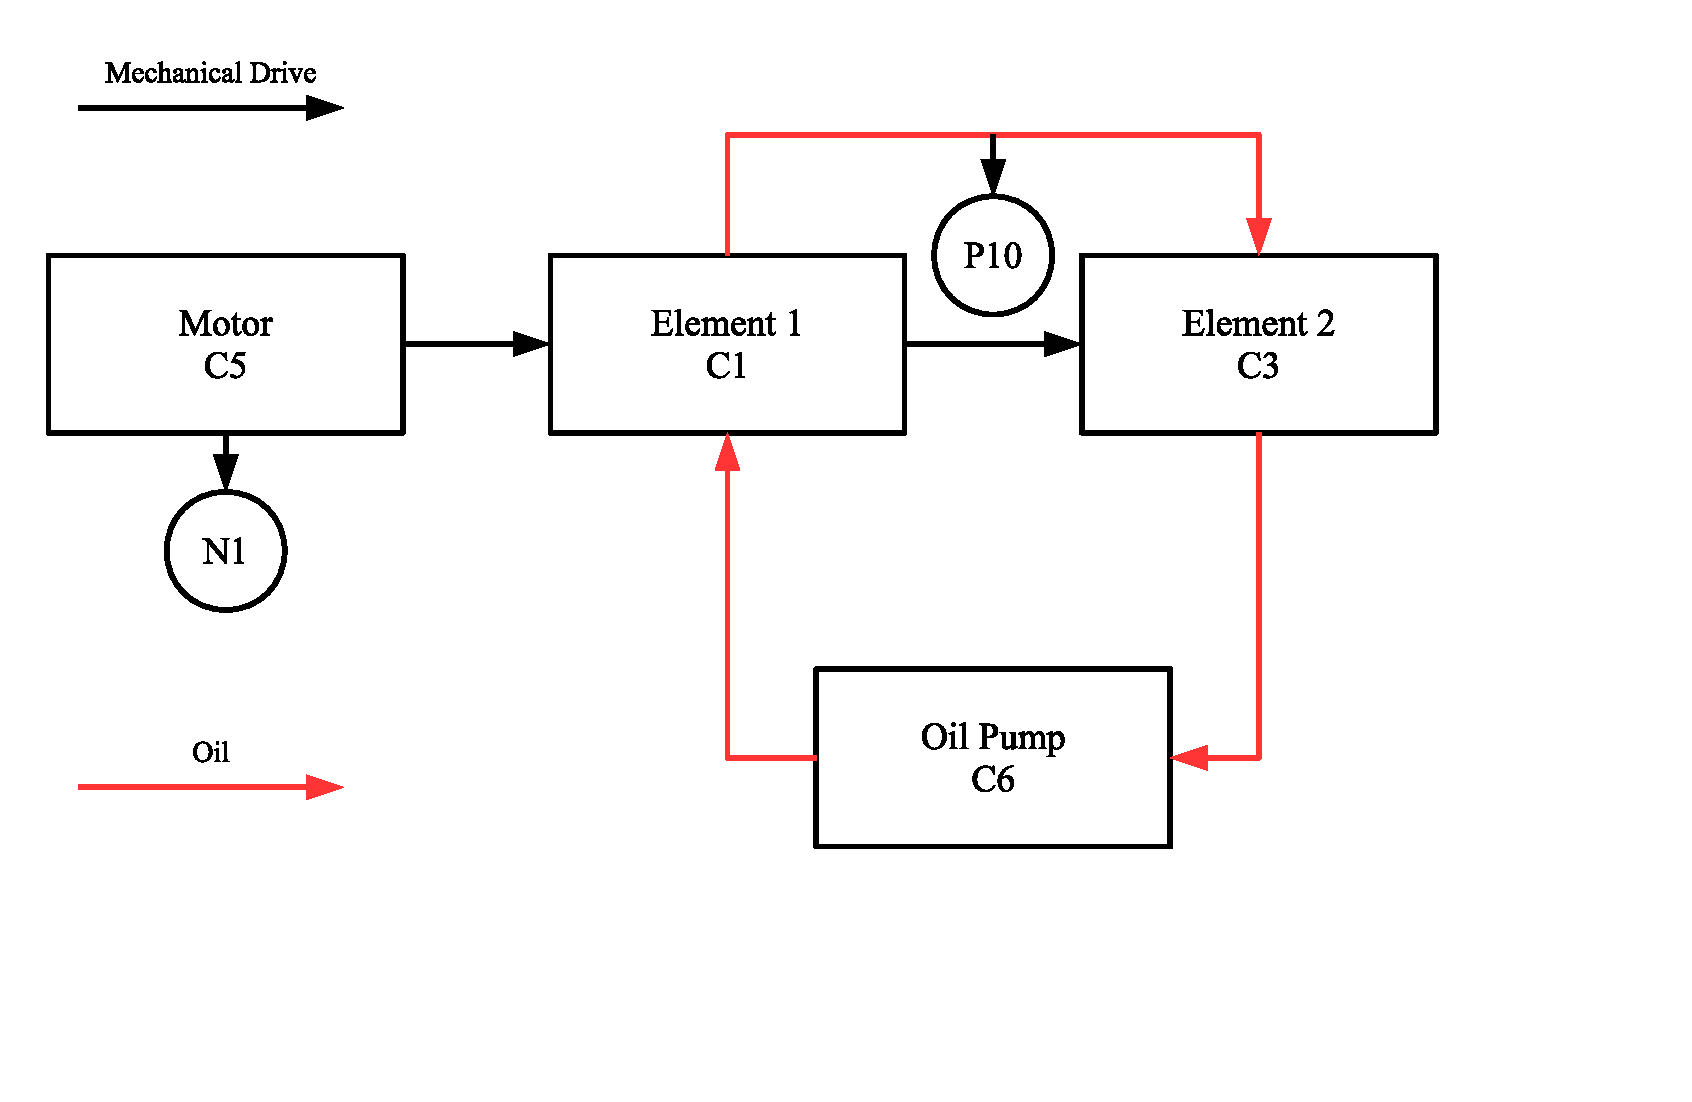
\includegraphics[width = \textwidth]{./Images/MechanicalCompressor.eps}
\caption{Mechanical drive two stage compressor}
\label{fig:mechcompressor}
\end{figure*}

   
% Table generated by Excel2LaTeX from sheet 'Sheet1'
\begin{table*}[htbp]
  \centering
  \scriptsize
  \caption{Compressor performance assessment rule set}
    \begin{tabular}{rlrrrrrrrrrrrrrrrr}
    \toprule
    \multicolumn{2}{c}{Rules} & \multicolumn{16}{c}{Potential Faults} \\
    \midrule
    ID    & Description & T1    & T2    & T3    & T4    & T5    & P1    & P2    & N1    & P10   & C1    & C2    & C3    & C4    & C5    & C6    & C7 \\
    \midrule
    1     & Element 1 Temperature Decrease & X     & X     &       &       &       &       &       &       &       & X     &       &       &       &       &       &  \\
    2     & Intercooler Temperature Increase &       & X     & X     &       &       &       &       &       &       &       & X     &       &       &       &       &  \\
    3     & Element 2 Temperature Decrease &       &       & X     & X     &       &       &       &       &       &       &       & X     &       &       &       &  \\
    4     & Aftercooler Temperature Increase &       &       &       & X     & X     &       &       &       &       &       &       &       & X     &       &       &  \\
    5     & Plant Room Temperature High & X     &       &       &       &       &       &       &       &       &       &       &       &       &       &       &  \\
    6     & Element 1 Outlet Temperature High &       & X     &       &       &       &       &       &       &       & X     &       &       &       &       &       &  \\
    7     & Element 2 Inlet Temperature High &       &       & X     &       &       &       &       &       &       &       & X     &       &       &       &       &  \\
    8     & Element 2 Outlet Temperature High &       &       &       & X     &       &       &       &       &       &       &       & X     &       &       &       &  \\
    9     & Final Outlet Temperature High &       &       &       &       & X     &       &       &       &       &       &       &       & X     &       &       &  \\
    10    & Expected Intercooler Pressure not Achieved &       &       &       &       &       & X     &       &       &       & X     &       &       &       &       &       &  \\
    11    & Increase in Outlet Pressure when Unloaded &       &       &       &       &       &       & X     &       &       &       &       &       &       &       &       & X \\
    12    & High Stop-Start Frequency of Motor Observed &       &       &       &       &       &       &       & X     &       &       &       &       &       & X     &       &  \\
    13    & Failure of Oil Pressure to Rise under Loading &       &       &       &       &       &       &       &       & X     &       &       &       &       &       & X     &  \\
    14    & Theoretical Element 1 Temperature Rise Exceeded &       & X     &       &       &       &       &       &       &       & X     &       &       &       &       &       &  \\
    15    & Theoretical Element 2 Temperature Rise Exceeded &       &       &       & X     &       &       &       &       &       &       &       & X     &       &       &       &  \\
    \bottomrule
    \end{tabular}%
  \label{tab:ruleset}%
\end{table*}%

% Table generated by Excel2LaTeX from sheet 'Naming Convention'
\begin{table}[htbp]
  \centering
  \caption{Rule set naming convention}
    \begin{tabular}{rr}
    \toprule
    Reference & Item \\
    \midrule
    T1    & Plant Room Temperature \\
    T2    & Element 1 Outlet Temperature \\
    T3    & Element 2 Inlet Temperature \\
    T4    & Element 2 Outlet Temperature \\
    T5    & Final Delivery Temperature \\
    P1    & Compressed Air Pressure in Intercooler  \\
    P2    & Compressed Air Final Delivery Pressure \\
    P3    & Compressed Air Receiver Pressure \\
    N1    & Motor starts per 5 minutes \\
    P10   & Oil Pressure \\
    P11   & Ambient Pressure \\
    C1    & Element 1 \\
    C2    & Intercooler \\
    C3    & Element 2 \\
    C4    & After Cooler \\
    C5    & Motor \\
    C6    & Oil Pump \\
    C7    & Load/Unload Valve \\
    \bottomrule
    \end{tabular}%
  \label{tab:namingconvention}%
\end{table}%




\lipsum[1-10]

\section{Operational mode identification}
\label{sec:modeidentification}

\section{Fault detection effectiveness}

\section{Conclusions and future work}
\label{sec:conclusions}


\section{Background: Air Compressor Operational Concerns}
\label{sec:1}
\section{Variable Speed Compressor Operational Modes}
\label{sec:2}
\section{Clustering for Mode Identification}
\label{sec:3}
It was noted during rule set development that it is desirable to know the mode of operation of an air compressor when applying rules. This follows on from lessons learned in similar work relating to HVAC \cite{Bruton2014}. With a HVAC unit, the different modes of operation that are useful to determine which rules to apply are heating only, heating with dehumidification, cooling, cooling with dehumidification and 

\section{Real-Time Analysis Implementation}
\label{sec:4}
\section{Results}
\label{sec:5}
\section{Discussion}
\label{sec:6}
\section{Conclusions}
\label{sec:7}


\section{Section title}
\label{sec:10}
Your text comes here. Separate text sections with
\section{Section X}
\label{sec:x}
Text with citations \cite{RefB} and \cite{RefJ}.
\subsection{Subsection title}
\label{sec:20}
as required. Don't forget to give each section 
and subsection a unique label (see Sect.~\ref{sec:1}).
\paragraph{Paragraph headings} Use paragraph headings as needed.
\begin{equation}
a^2+b^2=c^2
\end{equation}

% For one-column wide figures use
\begin{figure}
% Use the relevant command to insert your figure file.
% For example, with the graphicx package use
  
\includegraphics{example.eps}
% figure caption is below the figure
\caption{Please write your figure caption here}
\label{fig:1}       % Give a unique label
\end{figure}
%
% For two-column wide figures use
\begin{figure*}
% Use the relevant command to insert your figure file.
% For example, with the graphicx package use
  
\includegraphics[width=0.75\textwidth]{example.eps}
% figure caption is below the figure
\caption{Please write your figure caption here}
\label{fig:2}       % Give a unique label
\end{figure*}
%
% For tables use
\begin{table}
% table caption is above the table
\caption{Please write your table caption here}
\label{tab:1}       % Give a unique label
% For LaTeX tables use
\begin{tabular}{lll}
\hline\noalign{\smallskip}
first & second & third  \\
\noalign{\smallskip}\hline\noalign{\smallskip}
number & number & number \\
number & number & number \\
\noalign{\smallskip}\hline
\end{tabular}
\end{table}


%\begin{acknowledgements}
%If you'd like to thank anyone, place your comments here
%and remove the percent signs.
%\end{acknowledgements}
\newpage
% BibTeX users please use one of
\bibliographystyle{spbasic}      % basic style, author-year citations
%\bibliographystyle{spmpsci}      % mathematics and physical sciences
%\bibliographystyle{spphys}       % APS-like style for physics
\bibliography{JournalPaper1.bib}   % name your BibTeX data base

% Non-BibTeX users please use
%\begin{thebibliography}{}
%
% and use \bibitem to create references. Consult the Instructions
% for authors for reference list style.
%
%\bibitem{RefJ}
% Format for Journal Reference
%Author, Article title, Journal, Volume, page numbers (year)
% Format for books
%\bibitem{RefB}
%Author, Book title, page numbers. Publisher, place (year)
% etc
%\end{thebibliography}

\end{document}
% end of file template.tex

